\chapter{Beginning Combinatorics}

Discrete probability problems often include some counting. For
example, we figured out that there were 36 different ways the two dice, 
but all of them summed to some number 2 through 12. How
many different ways could three 8-sided dice come up? We would need to
count them, right? As the numbers get big we will need some tricks so
we don't need to write them all down and count them one-by-one.

The branch of mathematics that focuses on tricks for counting is
called \textit{combinatorics}.\index{combinatorics}
% KA: https://www.khanacademy.org/computing/pixar/crowds/crowds-1/v/combinatorics1

How can we be sure that there were 36 different configurations for the
two 6-sided dice? The first die could have come up as any one of six
numbers. For each of those, the second could have come up with any one
of six numbers. Thus, the number of possibilities is $ 6 \times 6 =
36.$

How many different configurations for 3 8-sided dice?  $8 \times 8
\times 8 = 8^3 = 512$.

What about seven dice, each with 20 sides? There would be $20^7=1,280,000,000$
configurations. See, aren't you glad we don't need to write them all
down?

Now, let's say that six people (Anne, Brock, Carl, Dev, Edgar, and Fred) are
going to run a race. You have to make a plaque that says who won first
place, who won second place, and who won third. If you want to get all
the possible plaques created beforehand, and just pull the right one
out as soon as the race ends, how many plaques would you need to get
engraved?

% 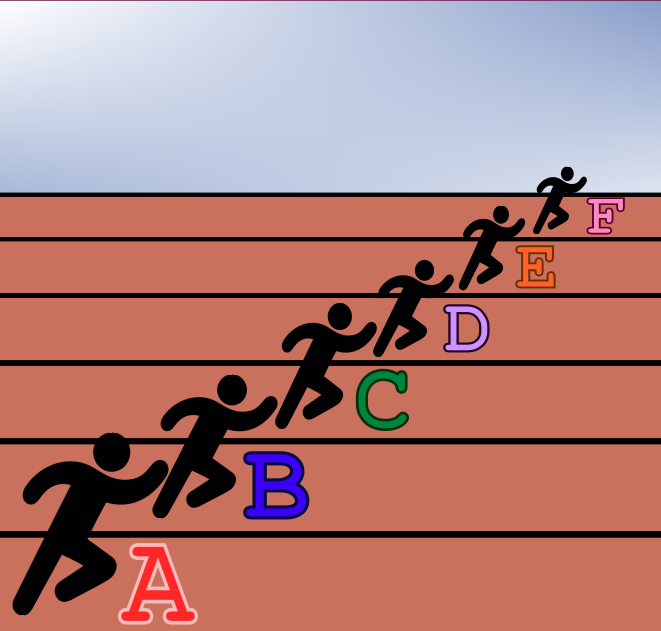
\includegraphics[width=0.8\textwidth]{Race.png}

In this case, once someone has been given first place, they can't win
second or third place. Thus, any of the 6 people can come in first,
but once you have engraved that person's name on the plaque, there are
only 5 people whose names can appear in second place. Once you have
engraved that name, there are only 4 people whose names can appear in
third place. Thus, you would get $6 \times 5 \times 4 = 120$ plaques
engraved.
% ADD: This situation is a little confusing given if they're doing the plaques before hand, they wouldn't know who came in each place

What if the plaque includes all 6 places?  Then you would need $6 \times 5
\times 4 \times 3 \times 2 \times 1 = 720$ plaques engraved.  We use
this process often enough that we gave it a name.  We say ``I need 6
factorial plaques engraved.''  When we write a factorial, we use an
exclamation point:\index{factorial}
% ADD: Same issue here

$$6! = 6 \times 5 \times 4 \times 3 \times 2 \times 1 = 720$$

We use the word ``permutation'' to mean a particular ordering.
This rule says $n$ items can be ordered in $n!$ ways. Thus
mathematicians actually say ``If you have a list of $n$ items then we
can generate $n!$ different permutations of those items''.

In Python, there is a \pyfunction{factorial} function in the math library:
\begin{Verbatim}[commandchars=\\\{\}]
> \textbf{python3} 
>>> \textbf{import math}
>>> \textbf{math.factorial(6)}
720
\end{Verbatim}

Handy, right? Now you don't need to write a loop to calculate factorials.

Remember when we only wanted the first three names on the plaque? We can do that problem using factorials:

$$6 \times 5 \times 4 = \frac{6 \times 5 \times 4 \times 3 \times 2 \times 1}{3 \times 2 \times 1} = \frac{6!}{3!}$$

This formulation makes it easy to figure out on any calculator with a ``!'' button.

The rule on this is to fill $m$ positions from $n$ items, it can be done this many ways:

$$\frac{n!}{(n-m)!}$$
% KA: https://www.khanacademy.org/computing/pixar/crowds/crowds2/v/combinatorics8

\subsection{Choose}

Let's say that there are 12 kids in a classroom, and you need a team
of 4 to wipe down the desks. How many different possible teams are
there? You know that if you were giving out four different positions
(Like the race gave out 1st, 2nd, and 3rd), the answer would be $12
\times 11 \times 10 \time 9$ or $12! / (12 - 4)!$.
% ADD: This is the probability that one person would be chosen

However, once we pick the 4 people, we don't care what order they are
in, right?  In this problem, the team ``Anne, Brad, Carl, and Don'' is
the same as the team ``Carl, Don, Brad, and Anne''.

Thus, the quantity $12! / (12 - 4)!$ is many times too large because
it counts each permutation separately. To get the right number, we
just divide this by the number of possible permuations for a group of
four people: $4!$

That gets us our answer: How many different teams of four can be chosen from 12 people?

$$\frac{12!}{(12-4)! 4!}= 495$$
% ADD: Needs a bit more explanation for claretiy, might just be my understanding
In combinatorics, we use this quantity a lot, so we have given it a name: \textit{choose}\index{choose function}

We have also given it a notation. ``12 choose 4'' is written like this:

$${12 \choose 4}$$
% KA Binomial Therom: https://www.khanacademy.org/math/precalculus/x9e81a4f98389efdf:series/x9e81a4f98389efdf:binomial/v/binomial-theorem

Python has the \pyfunction{math.comb} function:

\begin{Verbatim}[commandchars=\\\{\}]
> \textbf{python3}
>>> \textbf{import math}
>>> \textbf{comb(12, 4)}
495  
\end{Verbatim}

